\documentclass[12pt]{report}

\usepackage{graphicx}
\usepackage{textcomp}
\usepackage[margin=1.0in]{geometry}
\usepackage[symbol]{footmisc} % Used to have symbols for footnotes instead of numbers (so as to not get confused between references and footnotes)
\usepackage{gensymb} % Used for the degree symbol in math mode
\usepackage[subrefformat=parens,labelformat=parens]{subfig} % Used to combine figures into one\
\usepackage{bm} % Used for bold font in math mode
\usepackage{amsmath}
\usepackage{listings}
\usepackage{xcolor}
\usepackage{multirow}
\usepackage[superscript,biblabel,sort]{cite} % The superscript option puts the references as superscript numbers, biblabel applies the superscript to the references page, and sort sorts the numbers from least to greatest, and if possible, puts a dash to shorten it (i.e. 1,2,3,4,5,6 will be shortened to 1-6)
\usepackage{cleveref} % Makes references easier

\bibliographystyle{aip2}
% This is the methods section of the paper.
\begin{document}

\chapter{Methods}
Sufficient data is a requirement for any fitting procedure, but unfortunately there is a lack of data on UO\textsubscript{2} GB energies in the literature.  Molecular dynamics (MD) simulations were used to calculate the GB energies of various lattices based on the coincident site lattice (CSL) model to use as fitting data. This model is built off of the idea that GB energy is low when more lattice sites are in coincidence.  A number defined as the $\Sigma$-number describes the number of coincident sites per total sites in a given unit cell of a crystal.\cite{lejcek2010, rohrer2011} The data gathered was put into a MATLAB\textsuperscript{\textregistered} script developed using Bulatov \emph{et al.}'s methods\cite{bulatov2014} and building off of Harbison's\cite{harbison2015} script.  A reduced chi-square statistic was calculated to determine the effectiveness of the fit.

\section{Molecular Dynamics}
Simulation results from the Large-scale Atomic/Molecular Massively Parallel Simulation (LAMMPS) software (developed at Sandia National Laboratory\cite{plimpton1995}) were gathered for a number of twist, tilt, and mixed GBs.  These calculations were performed by creating two crystals of UO\textsubscript{2} and placing them together in various orientations.  A GB is introduced at the interface, creating GB energy.  The energy of the system is calculated from the interatomic forces inside the crystal.  That energy is compared to the energy of a single grain (of the same size as the combined two grains) of UO\textsubscript{2} in order to determine the energy at the GB.\cite{harbison2015}  The difference between these two values divided by twice the area of the GB gives the GB energy of the particular misorientation.\cite{butterfield2013} An example of how the atoms align is shown in \Cref{fig:lammps}. The original calculations as used by Harbison \cite{harbison2015} were done using no anneal (maximum temperature was approximately 0K), only allowing the atoms to relax to their local minima.  This work used an anneal of 800K, % NOTE: Why was 800K chosen?
allowing the atoms to relax to a better estimate of their global minimum value as is shown in \Cref{fig:100,fig:110,fig:111}.  
The misorientation angles at which these energies were calculated were the same as used in the work of Harbison.  These energies are used in the fitting procedure to produce parameters describing the five-dimensional GB space.
% This section needs more info, I just don't know what yet.  Mostly on MD information.  That would require some discussion with Yongfeng and Evan.

\begin{figure}[ht!]
 \centering
 
 \subfloat[]{\label{fig:lammps1}\includegraphics[scale=0.287]{"Images/LAMMPS example image"}}\quad
 \subfloat[]{\label{fig:lammps2}\includegraphics[scale=0.3]{"Images/LAMMPS example image2"}}\quad
 \caption{\label{fig:lammps}These figures demonstrate example crystal structures of UO\textsubscript{2} after an annealing process.  The better the atoms line up, the lower the energy is. \protect\subref{fig:lammps1} shows an example of a mostly aligned GB, indicative of a lower energy.  \protect\subref{fig:lammps2} shows an example of a misaligned GB, indicative of a higher energy.  These two images are from a \textlangle{}111\textrangle{} twist image.  Different viewpoints show different amounts of alignment.  The LAMMPS simulation package takes care of all the calculations to determine the energy at these GBs. Images courtesy of Dr. Evan Hansen, used with permission.}
\end{figure}

\section{Bulatov \emph{et al.}'s Methods}
In order to find the energy of an arbitrary GB in the five-space, Bulatov \emph{et al.}\cite{bulatov2014} implemented a hierarchical interpolation method.  They started by choosing three three-dimensional (3D) high-symmetry axes to use as scaffolding to build the entire five-dimensional (5D) function.  The axes chosen were the \textlangle{}100\textrangle{}, \textlangle{}110\textrangle{}, and the \textlangle{}111\textrangle{} sets for their four-, two-, and three-fold rotational symmetries respectively.\footnote{For cubic crystals, rotations of 90\textdegree{}, 180\textdegree{}, or 120\textdegree{} about any \textlangle{}100\textrangle{}, \textlangle{}110\textrangle{}, or \textlangle{}111\textrangle{} axis respectively is a symmetry operation.\cite{stokes2007}  Thus, the \textlangle{}100\textrangle{} set is four-fold symmetric (360\textdegree{}$/90$\textdegree{}$=4$), the \textlangle{}110\textrangle{} set is two-fold symmetric (360\textdegree{}$/180$\textdegree{}$=2$), and the \textlangle{}111\textrangle{} set is three-fold symmetric (360\textdegree{}$/120$\textdegree{}$=3$).}  Each 3D subset is built from an interpolation of their own one- and two-dimensional subsets.  The symmetric tilt and twist GBs for each set were fitted first because of their simplicity.  Only the rotation angle is needed to fully define the energies for these subsets, making them one-dimensional (in \Cref{fig:bulatov5D}, the darker bands in the smaller circles).  From the symmetric tilt subset, the asymmetric, or general, tilt subset was interpolated.  A second rotation angle defining the rotation of the second grain makes this subset two-dimensional (the lighter, wider band of color around the symmetric subset).  A combination of the general tilt subset (two dimensions) and the twist subset (one dimension) was used to interpolate the 3D subset for each high-symmetry axis (the three smaller circles).  These three 3D subsets were then used to interpolate the GB 5D space.

The equations used to do the interpolation were developed initially by Read and Shockley\cite{read1950} (called Read-Shockley functions) to describe the GB energy at low-angle boundaries (The definition of a ``low-angle boundary" varies from material to material.  Boundaries with angles higher than\cite{rohrer2011} 6\textdegree{} up to\cite{wolf1989} 15\textdegree{} have been cited as low-angle boundaries).  A method developed by Wolf\cite{wolf1989} used Read-Shockley functions to calculate the energies at high-angle boundaries, with the resulting functions being called Read-Shockley-Wolf (RSW) functions.  These RSW functions take the form:
\begin{equation}
E_{min} + (E_{max} - E_{min})\ \textnormal{sin}\left(\frac{\pi}{2}\frac{\theta-\theta_{min}}{\theta_{max} - \theta_{min}}\right)\left(1-a\textnormal{log}\left(\textnormal{sin}\left(\frac{\pi}{2}\frac{\theta-\theta_{min}}{\theta_{max} - \theta_{min}}\right)\right)\right),
\end{equation}
where $\theta$ is the misorientation angle, $\theta_{min}$ is the minimum angle on the domain, $\theta_{max}$ is the maximum angle on the domain, and $a$ is a shaping parameter.  Each RSW function as defined by Wolf covers a ``low-angle" subset of the domain of the 1D GB space.  An example of a simple RSW function is shown in \Cref{fig:RSW}.  Multiple RSW functions are stitched together to form the 1D subsets.

\begin{figure}[ht!]
 \centering
 \subfloat[]{\label{fig:bulatov5D}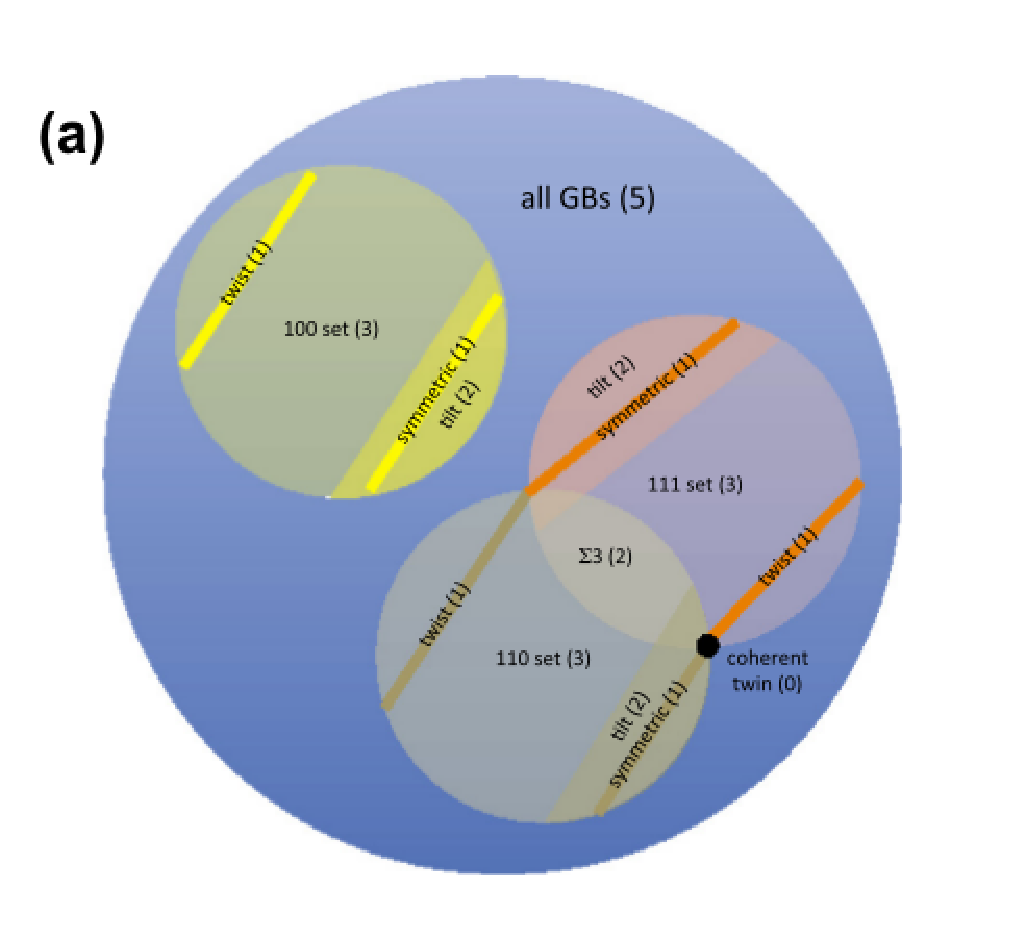
\includegraphics[scale=0.42]{Images/bulatov_5D_model}}\quad
 \subfloat[]{\label{fig:bulatovRodrigues}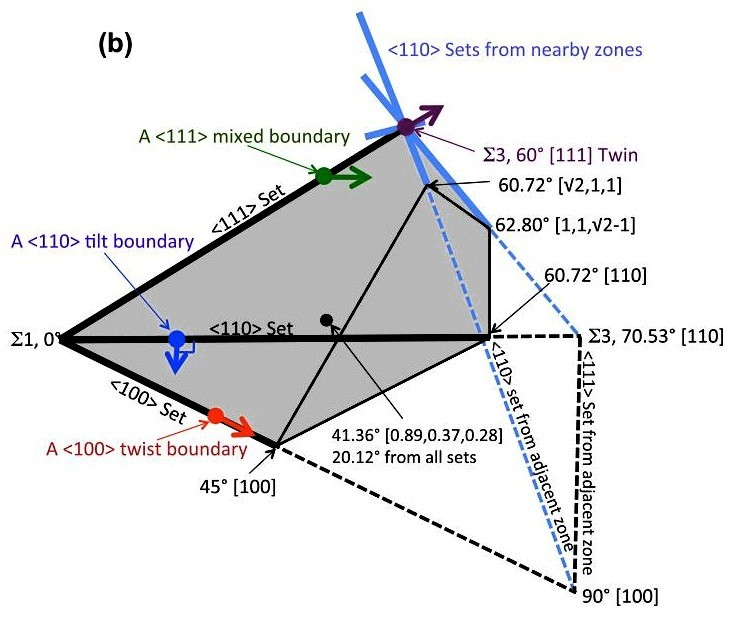
\includegraphics[scale=0.32]{Images/bulatov_rodrigues}}
 \caption{\label{fig:bulatovFig2}Figure 2 from Bulatov \emph{et al.}\cite{bulatov2014}. \protect\subref{fig:bulatov5D} demonstrates the theoretical relationship between the high-symmetry subsets of the 5D GB space.  Each multi-dimensional subset is interpolated from smaller-dimensional subsets. \protect\subref{fig:bulatovRodrigues} shows the Rodrigues space representation of the fundamental zone of all GBs as built from three high-symmetry axes (\textlangle{}100\textrangle{}, \textlangle{}110\textrangle{}, and \textlangle{}111\textrangle{}).  The unit vectors along the axis identify the boundary plane inclination in the frame of grain one.  A parallel vector thus represents a twist boundary, a perpendicular vector represents a tilt boundary, and neither parallel nor perpendicular vectors represent a mixed boundary.  The full misorientation space has 1152 symmetrically equivalent copies of the fundamental zone\cite{bulatov2014, randle2000} which allows the infinite nature of Rodrigues space to be accounted for.}
\end{figure}

\begin{figure}[ht!]
 \centering
 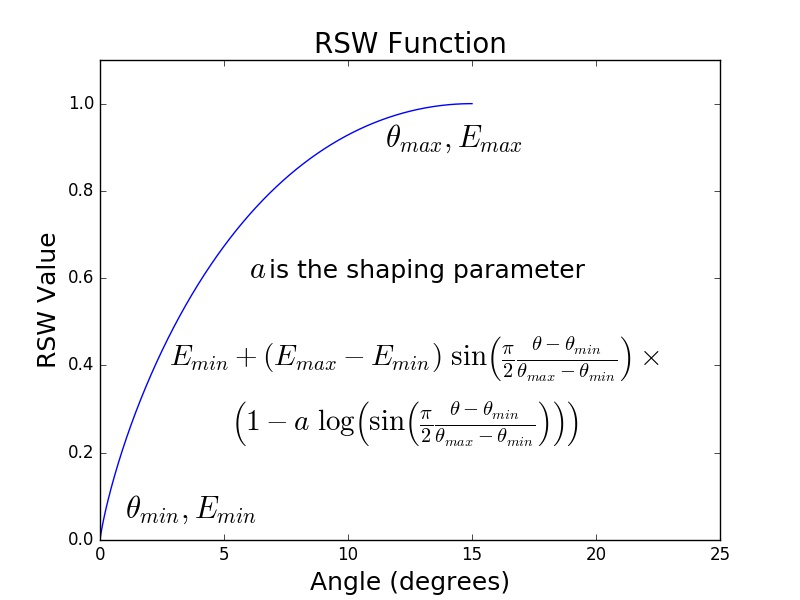
\includegraphics[scale=0.5]{Images/rsw}
 \caption{\label{fig:RSW}An example of an RSW function with $\theta_{min} = 0$\textdegree{}, $\theta_{max} = 15$\textdegree{}, and $a\ \textnormal{(the shaping parameter)} = 0.5$  Combining these functions into a Piecewise set over a given domain gives the GB energy curves their distinct, cusp-like behavior.  The RSW functions are scaled using $E_{min}$ and $E_{max}$.  In this example, $E_{min} = 0$ and $E_{max} = 1$.}
 % NOTE!!! using \degree WILL NOT WORK!
\end{figure}

\section{Representations of Grain Boundary Space}
Part of the development of this 5D function was accomplished through visual representations of the GB space.  However, the size of the five-space in which GBs reside makes representing them difficult.  Different methods have been developed to represent them, each with their advantages and disadvantages.  Three of these methods are the axis-angle representation, the Rodrigues representation, and the fundamental zone representation.  These methods, though described separately, can be used together to form a better picture of what the GB space looks like (see for example \Cref{fig:bulatovRodrigues} which combines the Rodrigues representation and the fundamental zone representation).

\subsection{Axis-Angle Representation}
The axis-angle representation is the simplest of the three described here.  The axis of rotation of the GB specifies the point in axis-angle space, and the angle of misorientation between the two grains at the GB specifies the magnitude of the vector.  Thus, mathematically representing an axis-angle vector is done by using the axis ($\bm{a}$, where $\bm{a}$ has components $a_x$, $a_y$, and $a_z$) and the angle ($\theta$) as:
\begin{equation}
\bm{A} = \bm{a}\ \theta
\label{eq:aaVec}
\end{equation} 

The axis-angle space can only take into account three degrees of freedom: the two angles specifying the axis, and the angle rotated through.  Thus, axis-angle space cannot fully visualize all of the necessary information contained in the full 5D space.\cite{frank1988} An added difficulty of using this representation is its infinite space because it is a mapping of an axis and an angle onto a Cartesian coordinate system.  This mapping means understanding the entire GB space is nearly impossible without the help of additional methods.  The axis-angle representation is best used as a starting point to move to other, more robust representations, and to represent the misorientation between two grains.\cite{randle2000}

\subsection{Rodrigues Representation}
The Rodrigues representation (sometimes called the ``Rodrigues-Frank" representation) uses Rodrigues vectors to represent rotations in Rodrigues space.  This representation takes ideas from the axis-angle space, but makes a few changes allowing crystal symmetries to be taken into account.  The axis about which a GB is oriented still specifies the point in space, but the magnitude of the vector is instead represented by the tangent of half the angle. Thus, a Rodrigues vector can be represented as:\cite{morawiec1996, becker1989, frank1988, randle2000, priester2013}
\begin{equation}
\bm{R}=\bm{a}\ \textnormal{tan}\left(\frac{\theta}{2}\right)
\label{eq:rodriguesVec}
\end{equation}
Some researchers favor this representation over others because of the lack of curvature such a mapping entails.\cite{frank1988, randle2000}  However, still only three of the five degrees of freedom are specified.  The other two are represented in \Cref{fig:bulatovRodrigues} by a unit vector at the point along the axis. A parallel vector represents a twist boundary, and a perpendicular vector represents a tilt boundary.  Anything else represents a mix of twist and tilt (or a mixed boundary).  One difficulty in using Rodrigues space is it also is an infinite space, as it simply maps an axis and an angle onto a Cartesian coordinate system.\cite{frank1988, kirch2008}.

\subsection{Fundamental Zone Representation}
The fundamental zone is perhaps the best graphical representation for the 5D GB.  This representation takes advantage of the symmetries inherent in crystals\cite{stokes2007} to simplify an infinite space into a compact, finite area called the fundamental zone.\cite{bulatov2014, patala2013, homer2015, morawiec1996, patala2012}  Every point within the space represents a unique orientation, and every point outside the space can be represented as a point inside the space through symmetry operations.\cite{morawiec1996, becker1989, frank1988}  Bulatov \emph{et al.} used this idea in connection with Rodrigues space to create \Cref{fig:bulatovRodrigues}.  In Rodrigues space, the fundamental zone is determine by the crystal symmetries of the material.\cite{patala2013, morawiec1996}  For fcc crystals, the fundamental zone takes the form of a truncated tetrahedron.\cite{bulatov2014}  The edges of the fundamental zone in Rodrigues space represent the high-symmetry rotation axes, and any point on the face of the fundamental zone can be represented by an equivalent points on another face.  

\section{Code Analysis}
Two MATLAB\textsuperscript{\textregistered} scripts created by Harbison\cite{harbison2015} and Bulatov \emph{et al.}\cite{bulatov2014} were used in this work.  These codes were analyzed to understand the process for both fitting the GB energy parameters, and for calculating the GB energy of an arbitrary GB.
\subsection{The Fitting Code}
An extensive analysis of the code written by Harbison\cite{harbison2015} to determine the parameters for the interpolation function was conducted to learn how the code worked.  The basic outline for how the fit occurs is as follows.  First, data is read in from a database containing energies associated with either a twist or tilt GB on one of the three high-symmetry axes.  Test parameters which are used as starting points are also read in from a separate database.  The one-dimensional sets are fitted first because of their simplicity.  The parameters found from the 1D fits are used in fitting the higher-dimensional sets.  Important angles are specified where low energies are expected, such as the $\Sigma5$ boundary for the \textlangle{}100\textrangle{} symmetric tilt subset.  These angles are calculated based on the $\Sigma$-number from CSL theory. Because the $\Sigma$-number designates how many lattice points  are between each coincident site (and assuming that the space between each lattice site, the lattice constant, is known) the angle of the GB misorientation can be determined.  In order to minimize the potential for error in calculations, every energy in the parameter-vector is listed as a scaled value based on the $e_{RGB}$ parameters -- a parameter representing the energy of an arbitrary, random GB, and can be seen as an average of the GB energies.  Thus, to make relevant comparisons, the energies are unscaled based on the units of energy desired (typically J/m\textsuperscript{2}).  An initial step size is then set, and data for the specific subsets is read in from a database.  All of the parameters and the angle-energy pairs are then passed into a grid-search fitting function.  Each subset had a different initial step size to avoid a numerical error where the steps would take the angles currently being looked at outside of their domain.

Once the six one-dimensional subsets and the three two-dimensional subsets are fitted, the three-dimensional subsets are fitted using the twist and asymmetric tilt subsets to calculate the mixing parameters (defining the relationship between the twist and general tilt subsets within a high-symmetry axis - i.e. the relationship between the small dark band of color representing the twist boundaries and the lighter, wider band of color representing the tilt boundaries in \Cref{fig:bulatov5D}).  The final step is to calculate the weighting parameters, which defines the relationship between the three high-symmetry subsets.  Equations defining the various relationships can be found in Bulatov \emph{et al.}'s work.

% I need to make sure I explain the difference between how the grid-search is calculating chi squared and how I calculated chi squared for our fit.  I should look into how Bulatov calculated his chi squared statistic.

\subsection{The Energy Calculation Code}
Bulatov \emph{et al.}'s open-source MATLAB\textsuperscript{\textregistered} code\cite{bulatov2014} calculates the energy of an arbitrary GB in an fcc metal. The same procedure is used for calculating an arbitrary GB in uranium dioxide, and goes as follows.  First, metrics defining the ``distance" between the GB and all three high-symmetry axes are calculated.  These distances are calculated by looking at all symmetrically equivalent representations of a GB on a per-axis basis (for cubic crystals, there are 24 equivalent representations\cite{stokes2007}).  Because there are 3, 6, and 4 unique axes for the \textlangle{}100\textrangle{}, \textlangle{}110\textrangle{}, and \textlangle{}111\textrangle{} axes respectively, a maximum of $6\times24=144$ distances are calculated.  Those distances exceeding a predefined cutoff distance are discarded, and after the loop going through each distance completes only the unique representations are kept to avoid double-counting certain representations.\cite{bulatov2014}  After these distances are calculated, energies are calculated for each unique distance in each set.  These energies are then weighted and summed together to give the interpolated energy for the specified GB. % This paragraph needs additional explanation on what the distances are.  What loop am I talking about?  I also use the phrase "Th[oe]se distances..." way too much.  This needs to be changed.

\section{Reduced Chi-Square Statistic}
A good way to test how well a function fits the data is to use a reduced chi-square goodness-of-fit statistic.\cite{bevington2003}  In order to get this statistic the orientation matrices (called the P and Q matrices by Bulatov \emph{et al.} for the first and second grain respectively) were needed as input parameters to the function provided by Bulatov.  These three by three matrices specify the orientation in a lab frame of the two grains individually. A good fit will have a reduced chi-square value close to one, while those values greater than one indicate an under fit, and those values less than one indicate an over fit.\cite{bevington2003}
\subsection{Developing the P and Q Matrices}
% This is going to need some major revisions
Creating the P and Q matrices was a non-trivial task.  Because there has been so much work done with crystallography over the past few decades, many different methods have been developed to specify the orientation matrices of grains. A rotation matrix also needed to be calculated which rotates the axis of rotation to the [100] direction, as assumed by Bulatov \emph{et al.}'s energy calculation code.  Three methods, following the method prescribed in MARMOT, using the Rodrigues rotation formula, and using the Bunge rotation matrix were used in the process of developing these matrices are described below.

\subsubsection{MARMOT Method}
MARMOT, Idaho National Laboratory's (INL's) mesoscale phase-field modeling platform,\cite{tonks2012} calculates the P and Q matrices for the grains using Euler angles as input parameters.  The Euler angles are converted to the orientation matrices using the Bunge convention, i.e. the $ZXZ$ or $ZX'Z''$ rotation, where the first rotation is about the \emph{z} axis, the second rotation is around the new \emph{x} axis, and the final rotation is about the new \emph{z} axis.  The formula for this conversion from Bunge Euler angles to the rotation matrix is found by multiplying the \emph{z} rotation matrix, \emph{x} rotation matrix, and \emph{z} rotation matrix together in that order to get:

\begin{equation}
\label{eq:bungeMat}
\left[
\begin{array}{ccc}
c_1\ c_3 - c_2\ s_1\ s_3 & -c_1\ s_3 - c_2\ c_3\ s_1 & \phantom{-}s_1\ s_2 \\
c_3\ s_1 + c_1\ c_2\ s_3 & \phantom{-}c_1\ c_2\ c_3 - s_1\ s_3 & -c_1\ s_2 \\
s_2\ s_3 & \phantom{-}c_3\ s_2 & \phantom{-}c_2 
\end{array}
\right]
\end{equation}
where $c_\textnormal{n}$ and $s_\textnormal{n}$ represent the cosine and sine of the respective angles (1 represents the first \emph{z} rotation, 2 represents the \emph{x} rotation, and 3 represents the second \emph{z} rotation.  These angles are usually referred to as\cite{randle2000} $\varphi_1$, $\Phi$, $\varphi_2$).

The rotation matrix was calculated in MARMOT by using the GB normal and finding the rotation matrix required to rotate that vector to the [100] direction.  In MARMOT simulations are set up through input files.  In the input files there are different blocks specifying material parameters, boundary conditions, initial conditions, and what physics to use to solve the problem (among others).  The initial condition used to calculate the rotation matrices in MARMOT was a horizontal or vertical line for tilt or twist boundaries respectively.  Because of this set up, the GB normals were either along the [010] axis for the tilt boundaries, or [$\bar{1}$00] for twist boundaries.

\subsubsection{Rodrigues Rotation Formula}
The Rodrigues rotation formula\cite{belongie2006} (RRF) is a way of calculating the rotation matrices given an axis and an angle using the following formula:
\begin{equation}
\label{eq:rrf}
\bm{R} = \bm{I} + \textnormal{sin}\ \theta\ \bm{K} + (1 - \textnormal{cos}\ \theta)\ \bm{K}^2,
\end{equation}
where $\bm{I}$ is the 3x3 identity matrix, $\theta$ is the angle rotated through, and $\bm{K}$ is the skew-symmetric matrix formed by the axis ($\bm{a}$) of rotation by:
\begin{equation}
\label{eq:skewSymMat}
\left[
\begin{array}{ccc}
\phantom{-}0 & -a_z & \phantom{-}a_y \\
\phantom{-}a_z & \phantom{-}0 & -a_x \\
-a_y & \phantom{-}a_x & \phantom{-}0
\end{array}
\right]
\end{equation}

The rotation matrices were calculated two different ways with this orientation matrix formulation.  One method was to simply use the MARMOT-generated rotation matrices.  These rotation matrices Another method was to calculate the rotation matrices using geometric arguments (see \Cref{fig:PlaneNorms}).  From these arguments the normals are identified in \Cref{table:geometricgbnorms}.

\begin{figure}[ht!]
\begin{minipage}{0.33\linewidth}
 \centering
 \subfloat[]{\label{fig:100TwistPlane}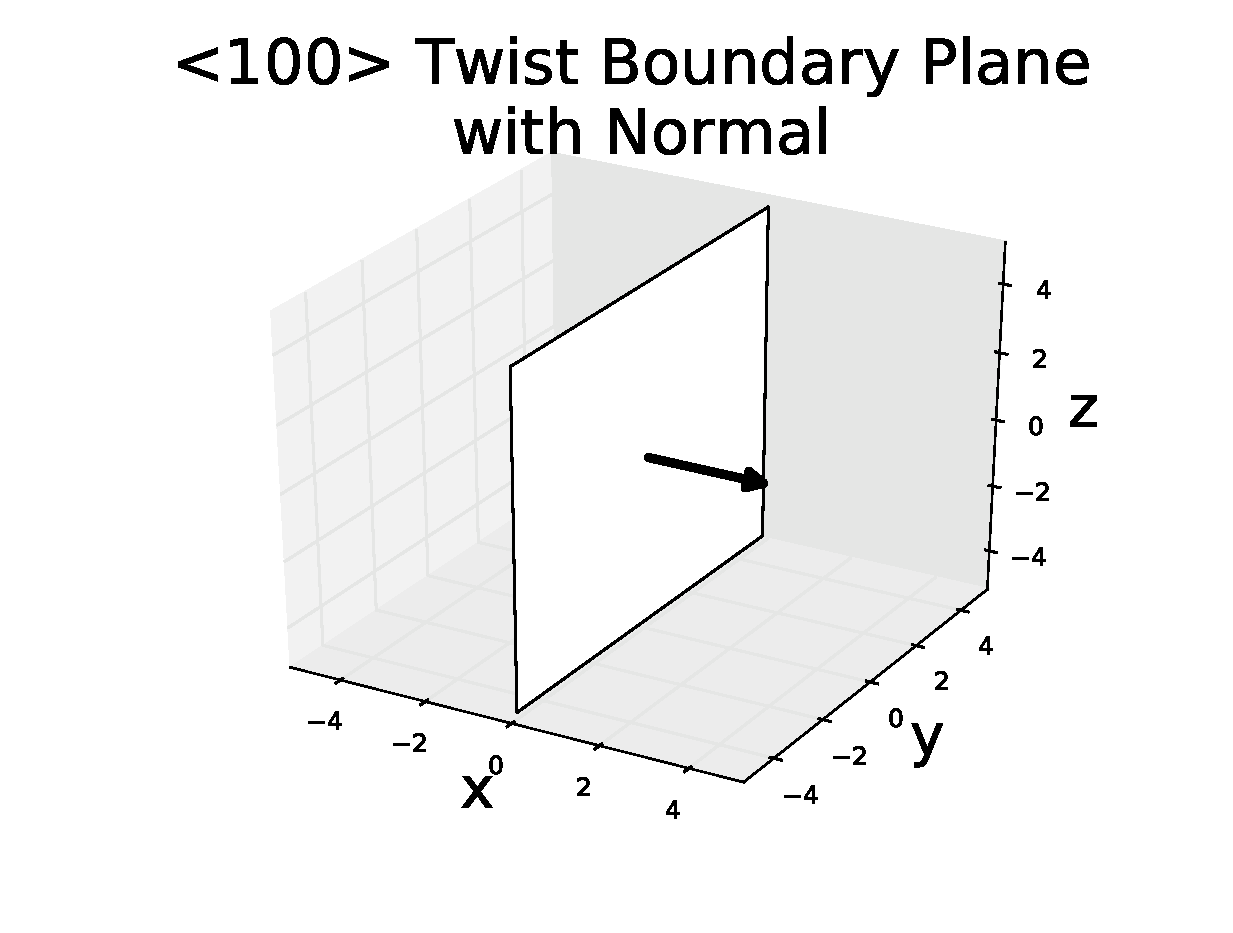
\includegraphics[scale=0.2]{Images/Twist100Plane}}
\end{minipage}%
\begin{minipage}{0.33\linewidth}
 \centering
 \subfloat[]{\label{fig:110TwistPlane}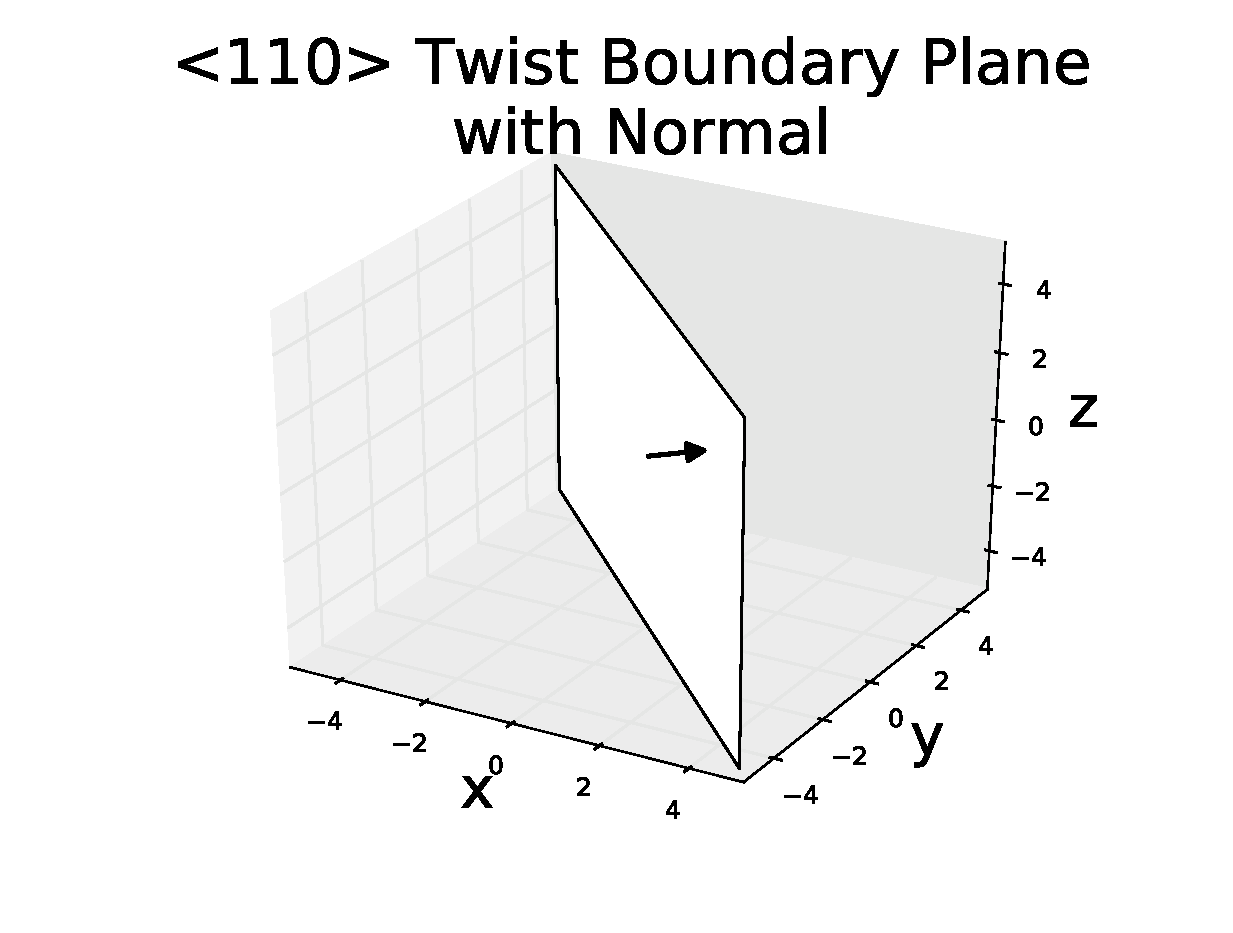
\includegraphics[scale=0.2]{Images/Twist110Plane}}
\end{minipage}%
\begin{minipage}{0.33\linewidth}
 \centering
 \subfloat[]{\label{fig:111TwistPlane}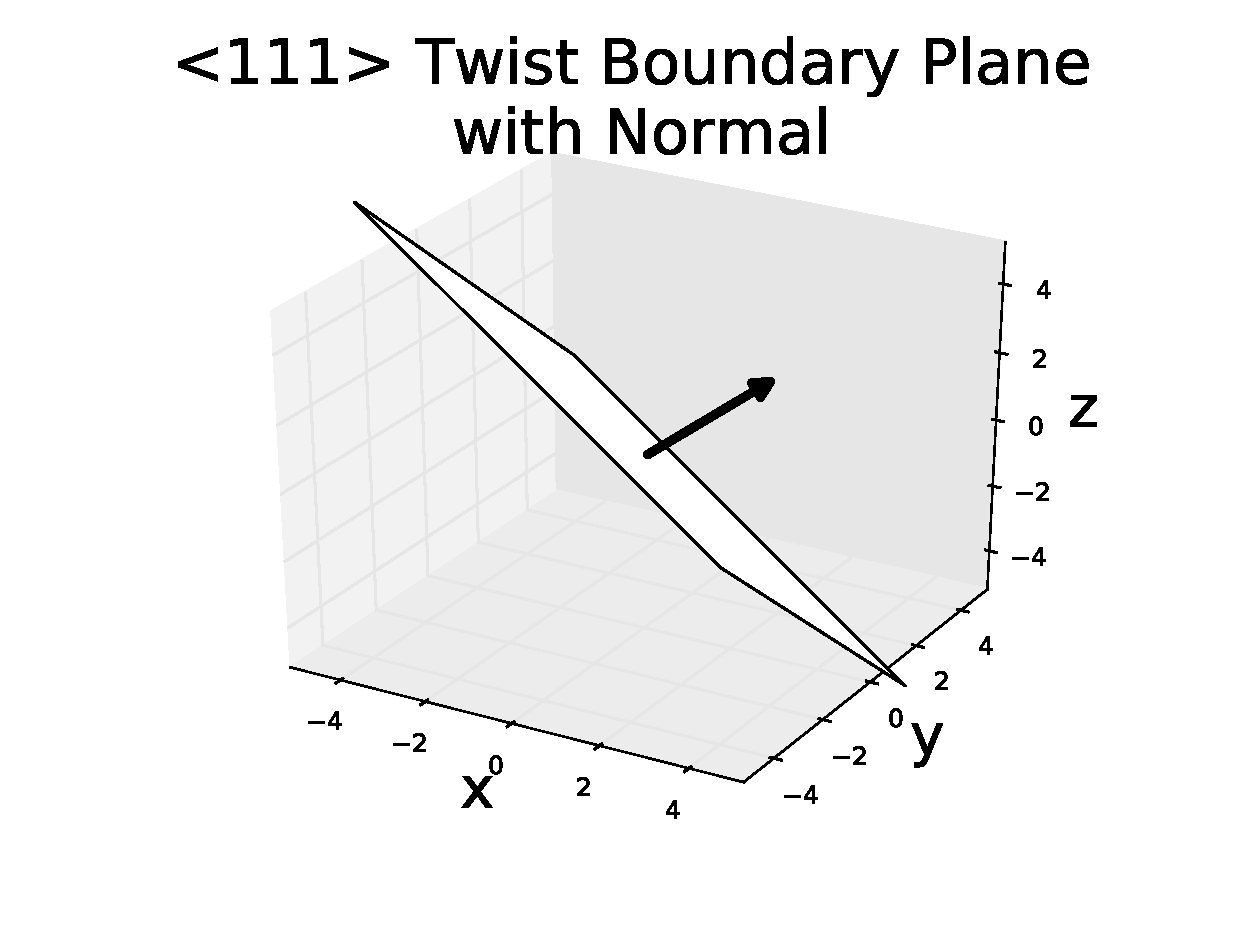
\includegraphics[scale=0.2]{Images/Twist111Plane}}
\end{minipage}
 \centering
 
 \subfloat[]{\label{fig:100TiltPlane}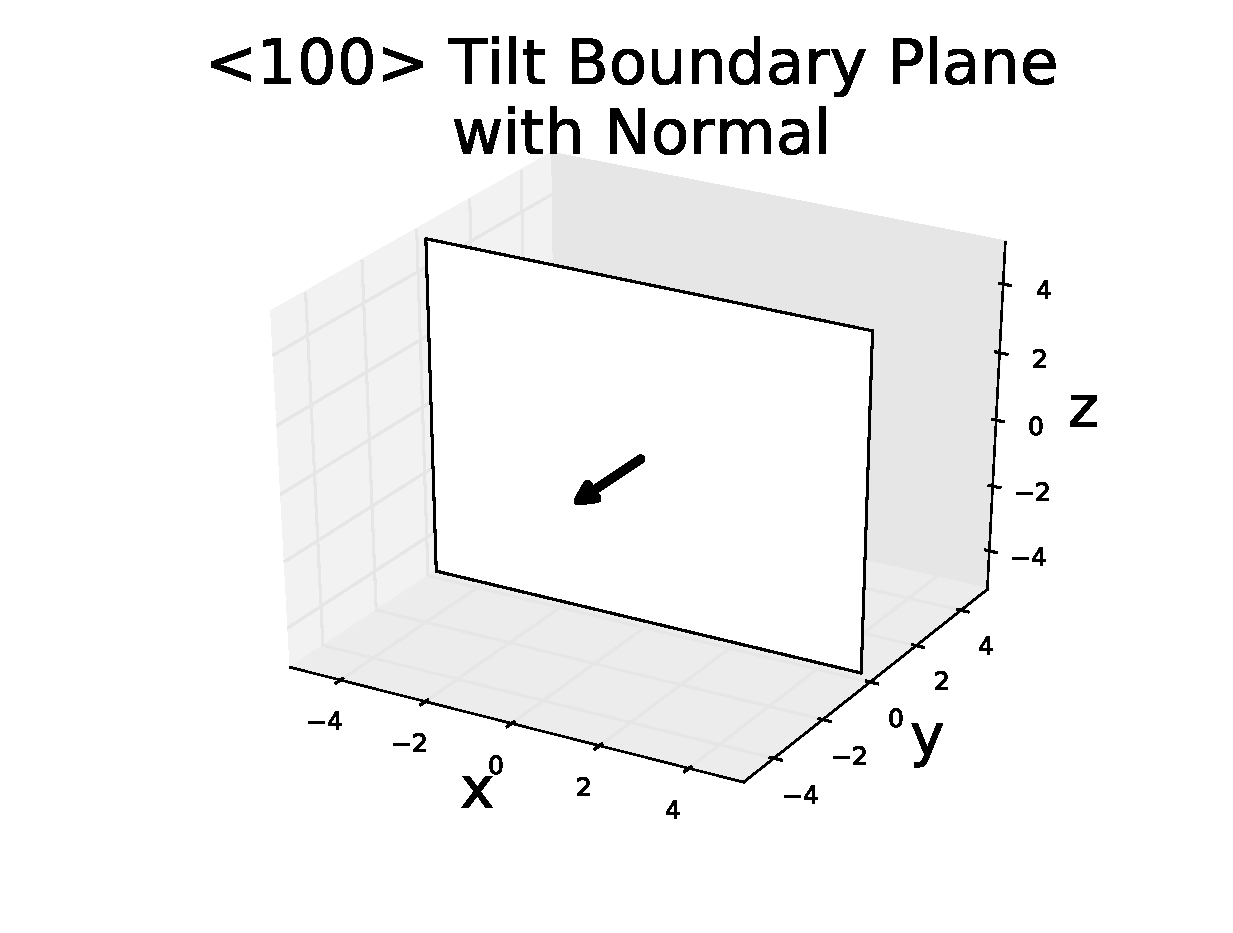
\includegraphics[scale=0.2]{Images/Tilt100Plane}}\quad
 \subfloat[]{\label{fig:110TiltPlane}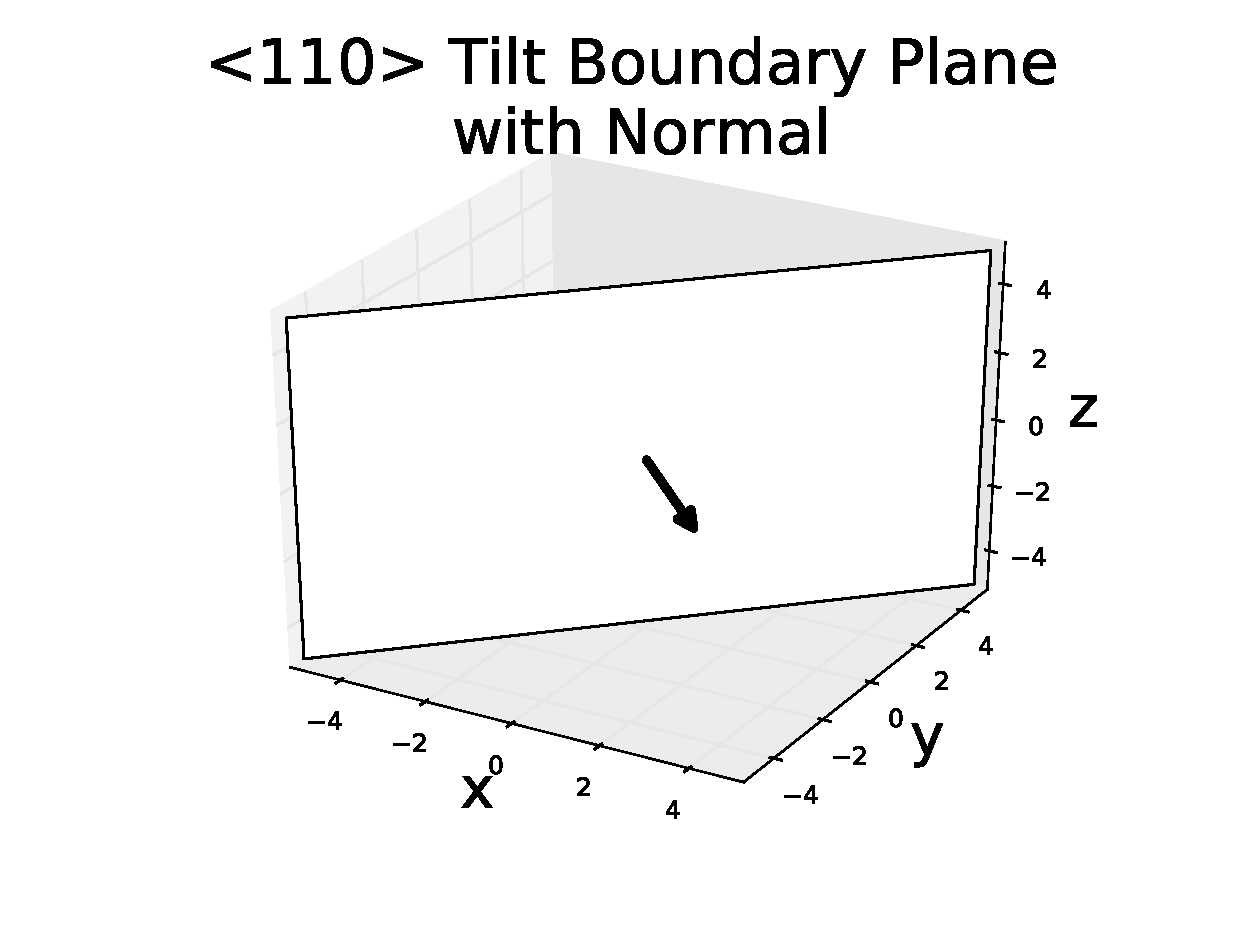
\includegraphics[scale=0.2]{Images/Tilt110Plane}}\quad
 \caption{\label{fig:PlaneNorms}A geometric method of determining the normals of a GB.  \protect\subref{fig:100TwistPlane} to \protect\subref{fig:111TwistPlane} show the GB normals for a GB perpendicular to the axis of rotation (a twist GB).  The GB normal is simply the axis about which the grains are rotated. \protect\subref{fig:100TiltPlane} and \protect\subref{fig:110TiltPlane} show the GB normals for a GB parallel to the axis of rotation (a tilt GB).  The GB normal is perpendicular to the axis of rotation.  The same GB normal for \textlangle{}110\textrangle{} Tilt can be used for \textlangle{}111\textrangle{} Tilt.}

\end{figure}

\begin{table}[ht!]
\centering
\caption{\label{table:geometricgbnorms}Table of GB normals for different GB types. The normalized dot product of the axis with the GB normal is zero in all tilt cases and one in all twist cases.  There are two options for the grain boundary normals of each subset because of inversion symmetries.}

\begin{tabular}{ccc}
\hline
Axis & Boundary Type & GB Normal \\
\hline
\multirow{2}{*}{\textlangle{}100\textrangle{}} & \multirow{2}{*}{Tilt} & [010] \\
                              & & [0$\bar{1}$0] \\
\multirow{2}{*}{\textlangle{}110\textrangle{}} & \multirow{2}{*}{Tilt} & [1$\bar{1}$0] \\
							  & & [$\bar{1}$10] \\
\multirow{2}{*}{\textlangle{}111\textrangle{}} & \multirow{2}{*}{Tilt} & [1$\bar{1}$0] \\
							  & & [$\bar{1}$10] \\
\multirow{2}{*}{\textlangle{}100\textrangle{}} & \multirow{2}{*}{Twist} & [100] \\
							  & & [$\bar{1}$00] \\
\multirow{2}{*}{\textlangle{}110\textrangle{}} & \multirow{2}{*}{Twist} & [110] \\
							  & & [$\bar{1}\bar{1}$0] \\
\multirow{2}{*}{\textlangle{}111\textrangle{}} & \multirow{2}{*}{Twist} & [111] \\
							  & & [$\bar{1}\bar{1}\bar{1}$] \\
\end{tabular}
\end{table}

\subsubsection{Bunge Rotation Matrix}
The Bunge rotation matrix is what was used by MARMOT (see \Cref{eq:bungeMat}) to create the orientation matrices.  There were various methods used to calculate the Euler angles, of which three are briefly described here. The Euler angles (once calculated) were used in the first two methods to calculate the entirety of the rotation matrix.

The first method tried was to use scripts developed to calculate the various Euler angles for MARMOT.  These scripts did not work because of the same assumptions made earlier about the orientation of the GB, namely, that all pure tilt GBs have a normal of 010, and that all pure twist GBs have a normal of $\bar{1}$00.  The difference between MARMOT's boundary conditions and the boundary conditions of this work is that GBs in this work are assumed to be either perpendicular or parallel to the rotation axis, as opposed to always being along the x or y axis.

The second method was to use an open-source MATLAB\textsuperscript{\textregistered} package called MTEX.\cite{bachmann2010}  This package calculates Euler angles using quaternions.  These Euler angles did not generate the correct results either, for the most part creating the same sorts of graphs as the MARMOT method.  It is uncertain why this method did not work.

The working method used the mathematics of quaternions.\cite{weisstein2004}  The quaternions were calculated directly based on the misorientation axis and angle.  A quaternion is a four-dimensional vector containing one real part, and three imaginary parts.  The components of the vector are calculated by:
\begin{equation}
\label{eq:quat}
\bm{q}=[\textnormal{cos}\frac{\theta}{2}, a_x \textnormal{sin}\frac{\theta}{2}, a_y \textnormal{sin}\frac{\theta}{2}, a_z \textnormal{sin}\frac{\theta}{2}],
\end{equation}
with axis $\bm{a}$ and misorientation angle $\theta$.  Once the axis and misorientation angle are converted to a quaternion, another conversion from a quaternion to the Bunge Euler angles is performed.  The angles are calculated using the \verb!atan2! method which allows for all four quadrants in the Cartesian space to be accounted for.  The angles are calculated using the following formulas:
\begin{align}
\label{eq:quat2euler}
\begin{aligned}
\chi &= \sqrt{(q_0^2+q_3^2)(q_1^2+q_2^2)}\\
\varphi_1 &= \textnormal{atan2}\left(\frac{(q_0q_2+q_1q_3)}{2\chi}, \frac{q_0q_1-q_2q_3}{2\chi}\right)\\
\Phi &= \textnormal{atan2}(2\chi, q_0^2+q_3^2-q_1^2-q_2^2)\\
\varphi_2 &= \textnormal{atan2}\left(\frac{(q_1q_3-q_0q_2)}{2\chi}, \frac{q_0q_1+q_2q_3}{2\chi}\right).
\end{aligned}
\end{align}
Once the Euler angles were calculated, they were put into \Cref{eq:bungeMat}, and the resulting matrices were used as the orientation for the grains.

\subsubsection{Testing The Matrices}
In order to test the different methods, an attempt was made to reproduce the 1D subset graphs as shown in Bulatov \emph{et al.}.  Various levels of success were observed for the different methods.  The matrices giving the best results are shown in \Cref{fig:reproduceBulatov100,fig:reproduceBulatov110,fig:reproduceBulatov111}.


While the first method works well for MARMOT, the challenge accompanying its use was that MARMOT specifies a specific GB normal with the set up of the problem that is not necessarily what is expected by the MATLAB\textsuperscript{\textregistered} script.  Thus, the results coming from using this combination of matrices ended up working only for the \textlangle{}100\textrangle{} tilt, \textlangle{}110\textrangle{} tilt, and \textlangle{}100\textrangle{} twist subsets, while the \textlangle{}110\textrangle{} twist had issues with singularities, and the \textlangle{}111\textrangle{} subsets did not remotely match the expected outcome.

\begin{figure}[ht!]
 \centering
 \subfloat[]{\label{fig:reproduceBulatov100Twist}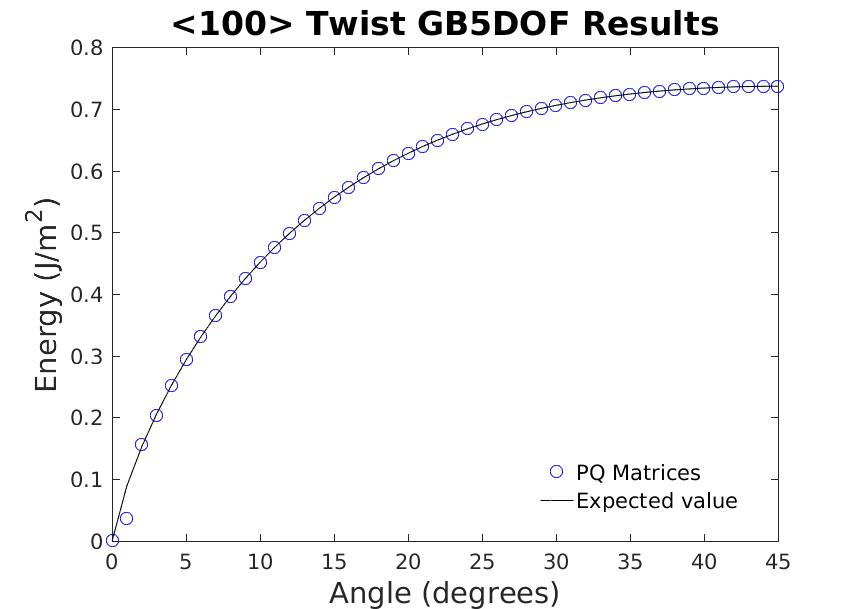
\includegraphics[scale=0.25]{Images/TestPQFit100Twist}}\quad
 \subfloat[]{\label{fig:reproduceBulatov100Tilt}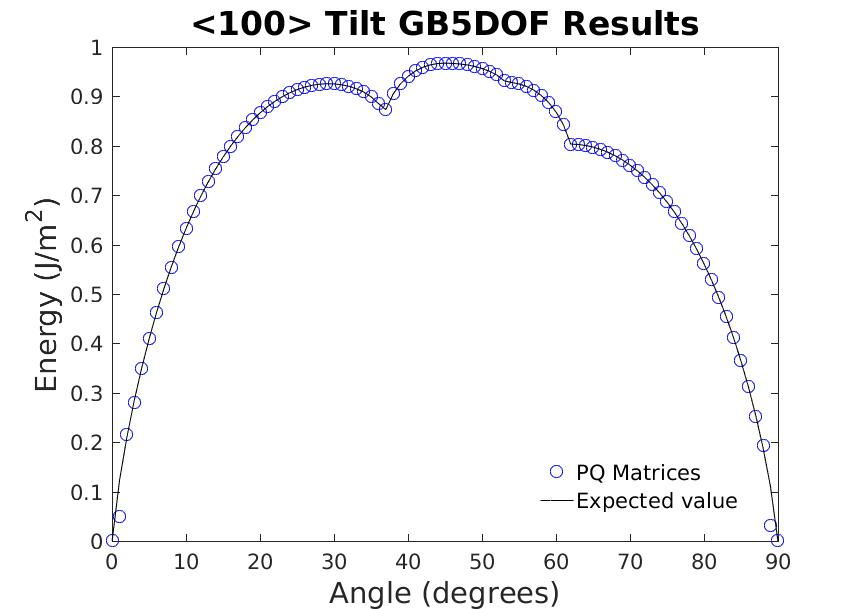
\includegraphics[scale=0.25]{Images/TestPQFit100Tilt}}\quad
 \caption{\label{fig:reproduceBulatov100} Results from using the P and Q matrices developed to re-create the \textlangle{}100\textrangle{} 1D subset figures shown in Bulatov \emph{et al.}  The expected value was calculated using Bulatov \emph{et al.}'s \lstinline!GB5DOF.m! MATLAB\textsuperscript{\textregistered} script with the default values, and the PQ Matrices values were calculated by inputting the matrices in the \lstinline!GB5DOF.m! script.  An inexact fit is found at the left end of both twist \protect\subref{fig:reproduceBulatov100Twist} and tilt \protect\subref{fig:reproduceBulatov100Tilt} profiles, and at the right edge of the tilt profile \protect\subref{fig:reproduceBulatov100Tilt}.  The interior of the domain fits exactly.  It is uncertain why the edges do not fit exactly.}
\end{figure}

\begin{figure}[ht!]
 \centering
 \subfloat[]{\label{fig:reproduceBulatov110Twist}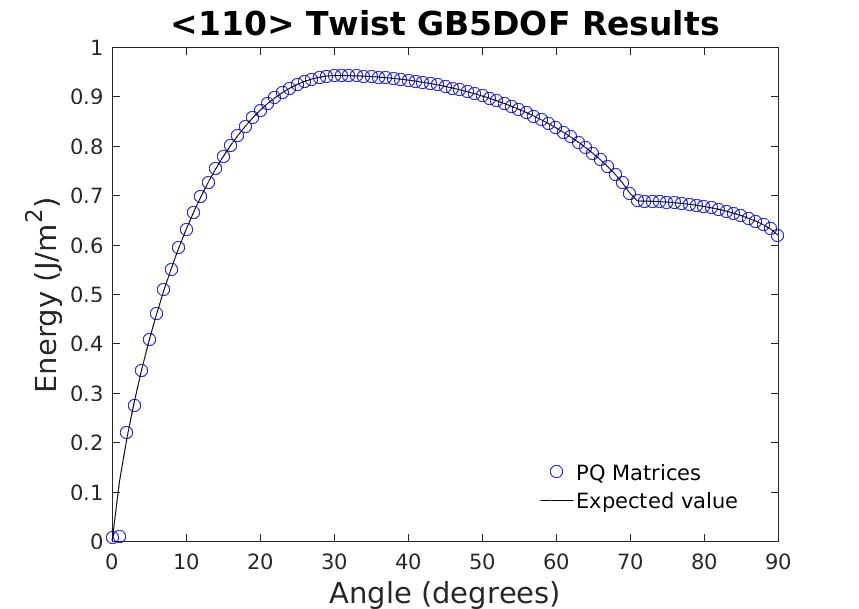
\includegraphics[scale=0.25]{Images/TestPQFit110Twist}}\quad
 \subfloat[]{\label{fig:reproduceBulatov110Tilt}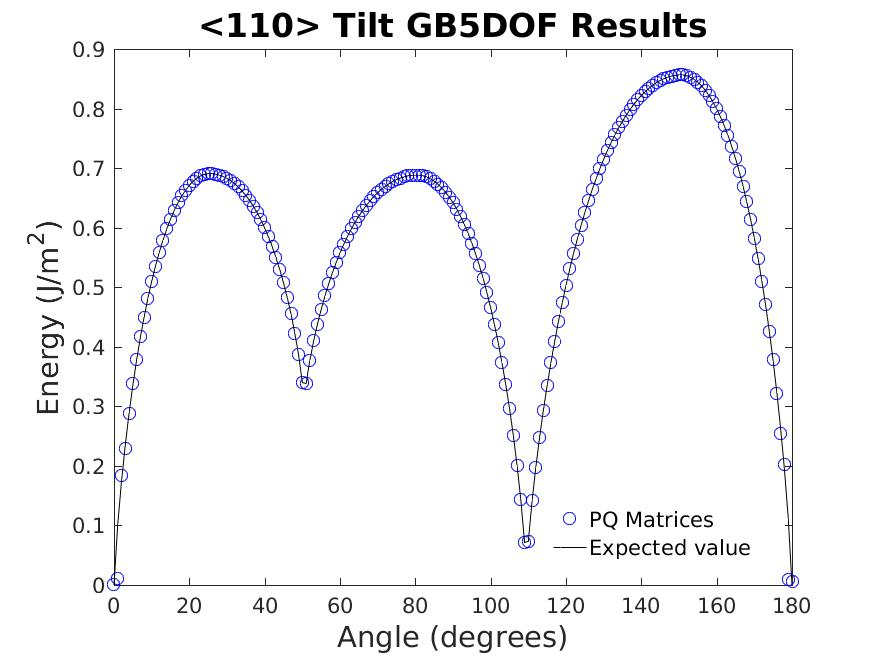
\includegraphics[scale=0.25]{Images/TestPQFit110Tilt}}\quad
 \caption{\label{fig:reproduceBulatov110} Results from using the P and Q matrices developed to re-create the \textlangle{}110\textrangle{} 1D subset figures shown in Bulatov \emph{et al.}  The expected value was calculated using Bulatov \emph{et al.}'s \lstinline!GB5DOF.m! MATLAB\textsuperscript{\textregistered} script with the default values, and the PQ Matrices values were calculated by inputting the matrices in the \lstinline!GB5DOF.m! script.  An inexact fit is found at the left end of both twist \protect\subref{fig:reproduceBulatov110Twist} and tilt \protect\subref{fig:reproduceBulatov110Tilt} profiles, and at the right edge of the tilt profile \protect\subref{fig:reproduceBulatov110Tilt}.  The interior of the domain fits exactly.  It is uncertain why the edges do not fit exactly.}
\end{figure}

\begin{figure}[ht!]
 \centering
 \subfloat[]{\label{fig:reproduceBulatov111Twist}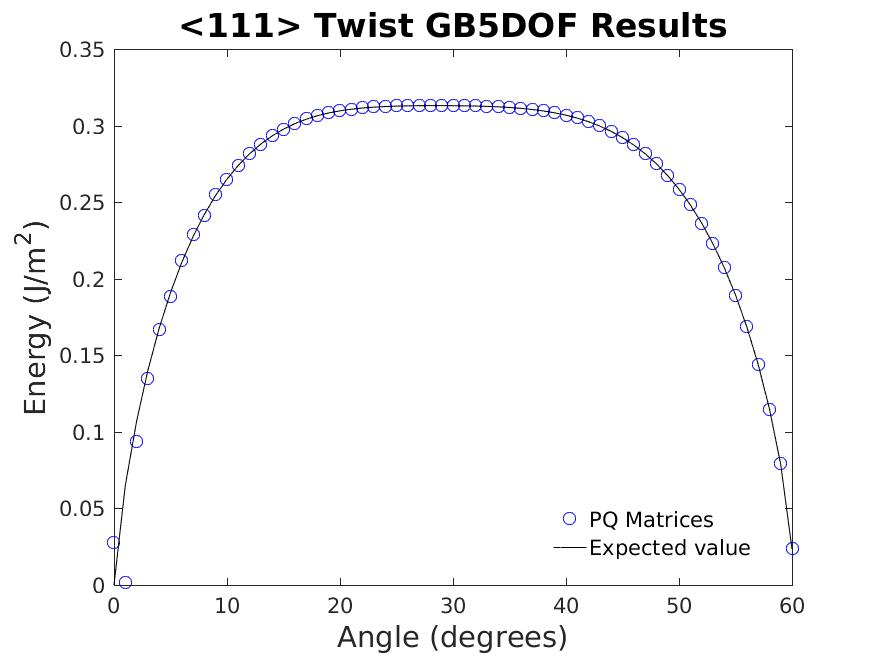
\includegraphics[scale=0.25]{Images/TestPQFit111Twist}}\quad
 \subfloat[]{\label{fig:reproduceBulatov111Tilt}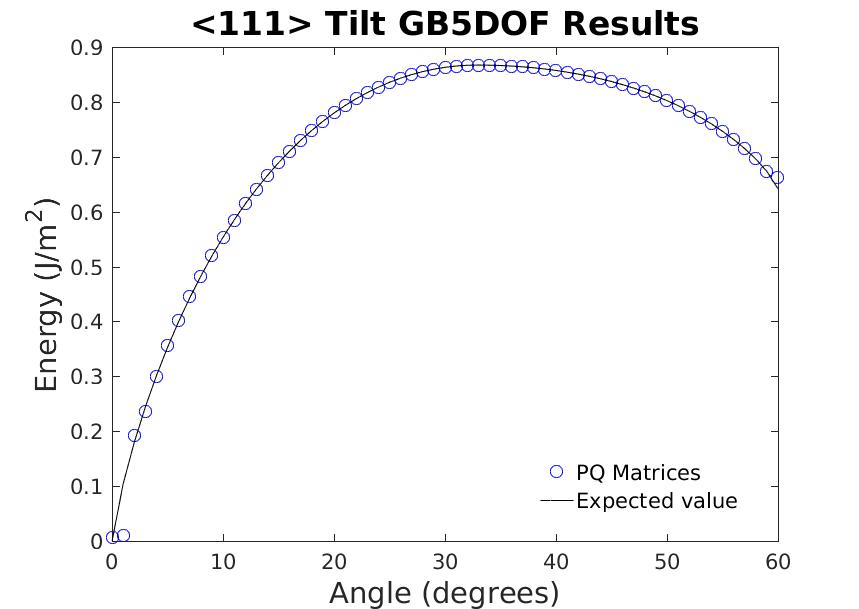
\includegraphics[scale=0.25]{Images/TestPQFit111Tilt}}\quad
 \caption{\label{fig:reproduceBulatov111} Results from using the P and Q matrices developed to re-create the \textlangle{}100\textrangle{} 1D subset figures shown in Bulatov \emph{et al.}  The expected value was calculated using Bulatov \emph{et al.}'s \lstinline!GB5DOF.m! MATLAB\textsuperscript{\textregistered} script with the default values, and the PQ Matrices values were calculated by inputting the matrices in the \lstinline!GB5DOF.m! script.  An inexact fit is found at the left end of both twist \protect\subref{fig:reproduceBulatov100Twist} and tilt \protect\subref{fig:reproduceBulatov100Tilt} profiles.  The interior of the domain fits exactly.  It is uncertain why the edges do not fit exactly.}
\end{figure}

\subsection{Calculating Reduced Chi Squared}
There were two methods used to calculate the $\chi^2_{red}$ statistic.  The first method was to use the P and Q matrices as developed above to test the entirety of the fit.  The second method was to calculate the statistic for each 1D subset, then calculate the full $\chi^2_{red}$ value using the statistics from the subsets.  Results from these calculations are discussed in the next chapter.

The test for the entire fit was done by using the P and Q matrices to calculate the energy in 1\textdegree{} intervals for each subset, using the \verb!GB5DOF.m! script.  The difference between the calculated values and the MD values was calculated, and the $\chi_{\textnormal{red}}^2$ value was calculated for each subset and for the entire fit, producing the results in \Cref{table:chi2} under the 800 K anneal column under the $\chi_{\textnormal{red}}^2$ using P and Q matrices section.

Using the second method, the same angles used in the fitting procedure were used in the RSW equations creating the 1D subsets.  The differences between the values resulting from there and the MD simulation values lead to the $\chi_{\textnormal{red}}^2$ values shown in the 800 K anneal column under the $\chi_{\textnormal{red}}^2$ comparing the 1D fits section.  The same methods were implemented to calculate the $\chi_{\textnormal{red}}^2$ values for the data without an anneal.

The statistic calculated using these methods is different from the $\chi^2$ statistic used in the grid-search function.  The grid search used \Cref{eq:chi2grid} shown below.

\begin{equation}
\label{eq:chi2grid}
\chi^2=\sum (E_{\textnormal{measured}} - E_{\textnormal{calculated}})^2
\end{equation}
\newpage
\bibliography{gbCharacter}
\end{document}